\documentclass[14pt, a4paper]{extarticle}

\usepackage[utf8]{inputenc}
\usepackage[T1]{fontenc}
\usepackage{amsmath}
\usepackage{amssymb}
\usepackage{graphicx}
\usepackage[left=2.00cm, right=2.00cm, top=2.00cm, bottom=2.00cm]{geometry}
\usepackage[russian]{babel}

\usepackage{setspace}
\usepackage{fancyhdr}

\graphicspath{{img/}}

\RequirePackage{caption}
\captionsetup[figure]{justification=centering,name=Рисунок,labelsep=endash}

\usepackage{indentfirst}

\usepackage{float}
\usepackage{listings}

\begin{document}
	\onehalfspacing
	\begin{titlepage}
	\begin{center}
		\begin{small}
			\textbf{Министерство науки и высшего образования Российской Федерации}

			ФЕДЕРАЛЬНОЕ ГОСУДАРСТВЕННОЕ АВТОНОМНОЕ ОБРАЗОВАТЕЛЬНОЕ УЧРЕЖДЕНИЕ ВЫСШЕГО ОБРАЗОВАНИЯ
			
			\textbf{<<НАЦИОНАЛЬНЫЙ ИССЛЕДОВАТЕЛЬСКИЙ УНИВЕРСИТЕТ ИТМО>>}
		\end{small}
		
		\vspace{8em}
		
		Отчет по лабораторной работе №4
		
		СИНТЕЗ ОПТИМАЛЬНОГО УПРАВЛЕНИЯ. ПРИНЦИП МАКСИМУМА
		
		По дисциплине <<Оптимальное управление>>
	\end{center}
	
	\vspace{8em}
	
	\begin{flushright}
		Выполнил:\\
		студент группы R42331c\\
		Манахов~С.П.
		
		\vspace{1em}
		
		Преподаватель:\\
		Парамонов~А.В.
	\end{flushright}

	\vfill
	
	\begin{center}
		\small
		Санкт-Петербург\\
		2022 г.\\
	\end{center}
\end{titlepage}
	\setcounter{page}{2}

	\section*{Задание}
	
	Найти минимум критерия качества для статической задачи оптимизации:
	\begin{enumerate}
		\item Поиск глобального минимума $J(x,u)$ на основе необходимого и достаточного условия:
		\begin{enumerate}
			\item[1.1] Без ограничений;
			\item[1.2] С ограничением в виде равенства $c(x,u)=0$;
			\item[1.3] С ограничением в виде неравенства $c(x,u)\le0$; 
		\end{enumerate}
		\item Градиентный поиск минимума критерия качества:
		$$J_1(x,u)=J(x,u)$$
		\begin{enumerate}
			\item[2.1] Методом Ньютона Рафсона произвести пошаговый расчет экстремума;
			\item[2.2] Методом наискорейшего спуска для двух различных $\gamma$ (соответствующей колебательной и апериодической сходимости) произвести пошаговый расчет экстремума. 
		\end{enumerate}
	\end{enumerate}
	\begin{table}[H]
		\centering
		\begin{tabular}{|c|c|c|}
			\hline
			Вариант & $J(x,u)$ & $c(x,u)$ \\\hline
			9 & $J(x,u)=4x^2+5u^2+7xu+5x+6u-8$ & $x-u^2-8$ \\\hline
		\end{tabular}
	\end{table}
	
	\newpage
	
	\section*{Описание работы}
	
	Для поиска глобального минимума $J(x,u)$ без ограничений составим градиент:
	$$gradJ(x,u)=\nabla J(x,u)=\left[\begin{matrix}
		\frac{\partial J(x,u)}{\partial x} \\
		\frac{\partial J(x,u)}{\partial u} \\
	\end{matrix}\right]=\left[\begin{matrix}
		8x+7u+5 \\
		10u+7x+6 \\
	\end{matrix}\right]$$
	
	Приравняем каждый элемент градиента к нулю и решим следующую систему уравнений:
	$$\begin{cases}
		8x+7u+5=0 \\
		10u+7x+6=0 \\
	\end{cases}$$
	Откуда следует, что $x=-\frac{8}{31}$ и $u=-\frac{13}{31}$, подставим в выражение для критерия качества и получим:
	$$J_{min}=-\frac{307}{31}=-9,9032$$
	
	Для поиска глобального минимума $J(x,u)$ с ограничением в виде равенства $c(x,u)=0$ составим лагранжиан:
	$$L(x,u,\lambda)=J(x,u) + \lambda c(x,u) = 4x^2+5u^2+7xu+5x+6u-8 + \lambda (x-u^2-8)$$
	
	Также найдем градиент и приравняем каждый элемент к нулю:
	$$\begin{matrix}
		\begin{cases}
			\frac{\partial L}{\partial \lambda}=0 \\
			\frac{\partial L}{\partial x}=0 \\
			\frac{\partial L}{\partial u}=0 \\
		\end{cases} &
		\begin{cases}
			x-u^2-8 = 0 \\
			8x+7u+5+\lambda = 0 \\
			10u+7x+6-2\lambda u = 0
		\end{cases}
	\end{matrix}$$
	Учитывая только действительные значения, получаем, что $x=8,1910$, $u=-0,4370$ и $\lambda=-67,4688$. Подставим в выражение для критерия качества:
	$$J_{min} = 274,5994$$
	
	Для поиска глобального минимума $J(x,u)$ с ограничением в виде неравенства $c(x,u)\le0$ составим и решим следующую систему:
	$$\begin{cases}
		x-u^2-8 \le 0 \\
		8x+7u+5+\lambda = 0 \\
		10u+7x+6-2\lambda u = 0
	\end{cases}$$
	Учитывая только действительные значения, получаем, что $x=-\frac{8}{31}$, $u=-\frac{13}{31}$ и $\lambda=0$. Подставим в выражение для критерия качества:
	$$J_{min}=-9,9032$$
	Отметим, что при этом выполняются условие Куна-Таккера $\lambda\le0$ и условие дополняющей нежёсткости $\lambda c(x,u)=0$.
	
	Осуществим градиентный поиск минимума критерия качества методом Ньютона Рафсона по следующей формуле:
	$$\bar{X}^{(n+1)}=\bar{X}^{(n)}-H^{-1}(\bar{X}^{(n)})\nabla J(\bar{X}^{(n)})$$
	где:
	$$\begin{matrix}
		\bar{X}^{(n)} = 
		\left[\begin{matrix}
			x(n) \\ u(n)
		\end{matrix}\right], &
		\nabla J(\bar{X}^{(n)})= 
		\left[\begin{matrix}
			\frac{\partial J(\bar{X}^{(n)})}{\partial x} \\
			\frac{\partial J(\bar{X}^{(n)})}{\partial u} \\
		\end{matrix}\right] = 
		\left[\begin{matrix}
			8x(n)+7u(n)+5 \\
			10u(n)+7x(n)+6 \\
		\end{matrix}\right]
	\end{matrix}$$
	$$H(\bar{X}^{(n)})= 
	\left[\begin{matrix}
		\frac{\partial}{\partial x}\left(\frac{\partial J(\bar{X}^{(n)})}{\partial x}\right) &
		\frac{\partial}{\partial x}\left(\frac{\partial J(\bar{X}^{(n)})}{\partial u}\right) \\
		\frac{\partial}{\partial u}\left(\frac{\partial J(\bar{X}^{(n)})}{\partial x}\right) &
		\frac{\partial}{\partial u}\left(\frac{\partial J(\bar{X}^{(n)})}{\partial u}\right) \\
	\end{matrix}\right]=
	\left[\begin{matrix}
		8 & 7 \\ 7 & 10 
	\end{matrix}\right]$$
	
	Начинать поиск будем с найденных в пункте~1.2 значений: $x(1)=8,1910$, $u(1)=-0,4370$.
	
	Минимум найден за один шаг:
	$$\begin{matrix}
		x(2)=-0,2581; & u(2)=-0,4194; & J(2)=J_{min}=-9,9032
	\end{matrix}$$
	
	Осуществим градиентный поиск минимума критерия качества методом наискорейшего спуска по следующей формуле:
	$$\bar{X}^{(n+1)}=\bar{X}^{(n)}-\gamma\nabla J(\bar{X}^{(n)})$$
	
	Будем использовать скрипт, представленный ниже:
	\begin{small}
		\lstinputlisting[language=Matlab]{m/lab1_2a.m}
	\end{small}
	
	С коэффициентом $\gamma=0,1$ минимум найден за 31~итерацию:
	$$\begin{matrix}
		x(32)=-0,2518; & u(32)=-0,4248; & J(32)=J_{min}=-9,9032
	\end{matrix}$$
	
	На рисунке \ref{fig:gamma01} представлен результат работы алгоритма, соответствующий колебательной сходимости.
	
	\begin{figure}[H]
		\centering
		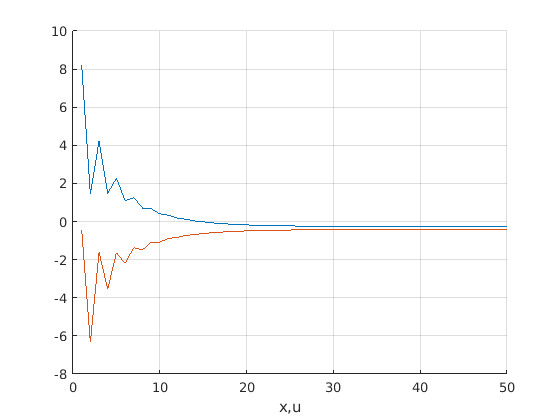
\includegraphics[width=0.6\textwidth]{gamma01}
		\caption{Значения $x,u$ при $\gamma=0,1$}
		\label{fig:gamma01}
	\end{figure}
	
	С коэффициентом $\gamma=0,066$ минимум найден за 49~итераций:
	$$\begin{matrix}
		x(50)=-0,2520; & u(50)=-0,4247; & J(50)=J_{min}=-9,9032
	\end{matrix}$$

	На рисунке \ref{fig:gamma0066} представлен результат работы алгоритма, соответствующий апериодической сходимости.
	
	\begin{figure}[H]
		\centering
		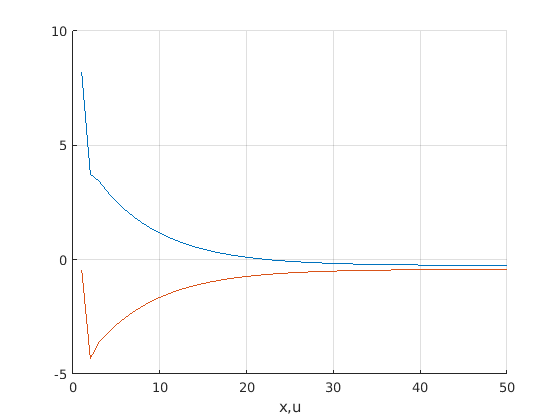
\includegraphics[width=0.6\textwidth]{gamma0066}
		\caption{Значения $x,u$ при $\gamma=0,066$}
		\label{fig:gamma0066}
	\end{figure}

	\newpage
	
	\section*{Вывод}
	
	С увеличением числа наложенных ограничений процесс поиска минимума критерия качества $J(x,u)$ усложняется.
	
	Среди методов градиентного поиска самым быстрым оказался метод Ньютона Рафсона, но он требует вычисления матрицы Гессе, что может замедлить процесс поиска, в отличии от метода наискорейшего спуска, который требует только вычисления градиента.
	
\end{document}